\begin{figure}
\captionsetup[subfigure]{justification=centering}
\centering
\begin{tabular}{ccc}
\subcaptionbox{Belonging screen\label{fig:cross-device:sga50:belonging}}{ 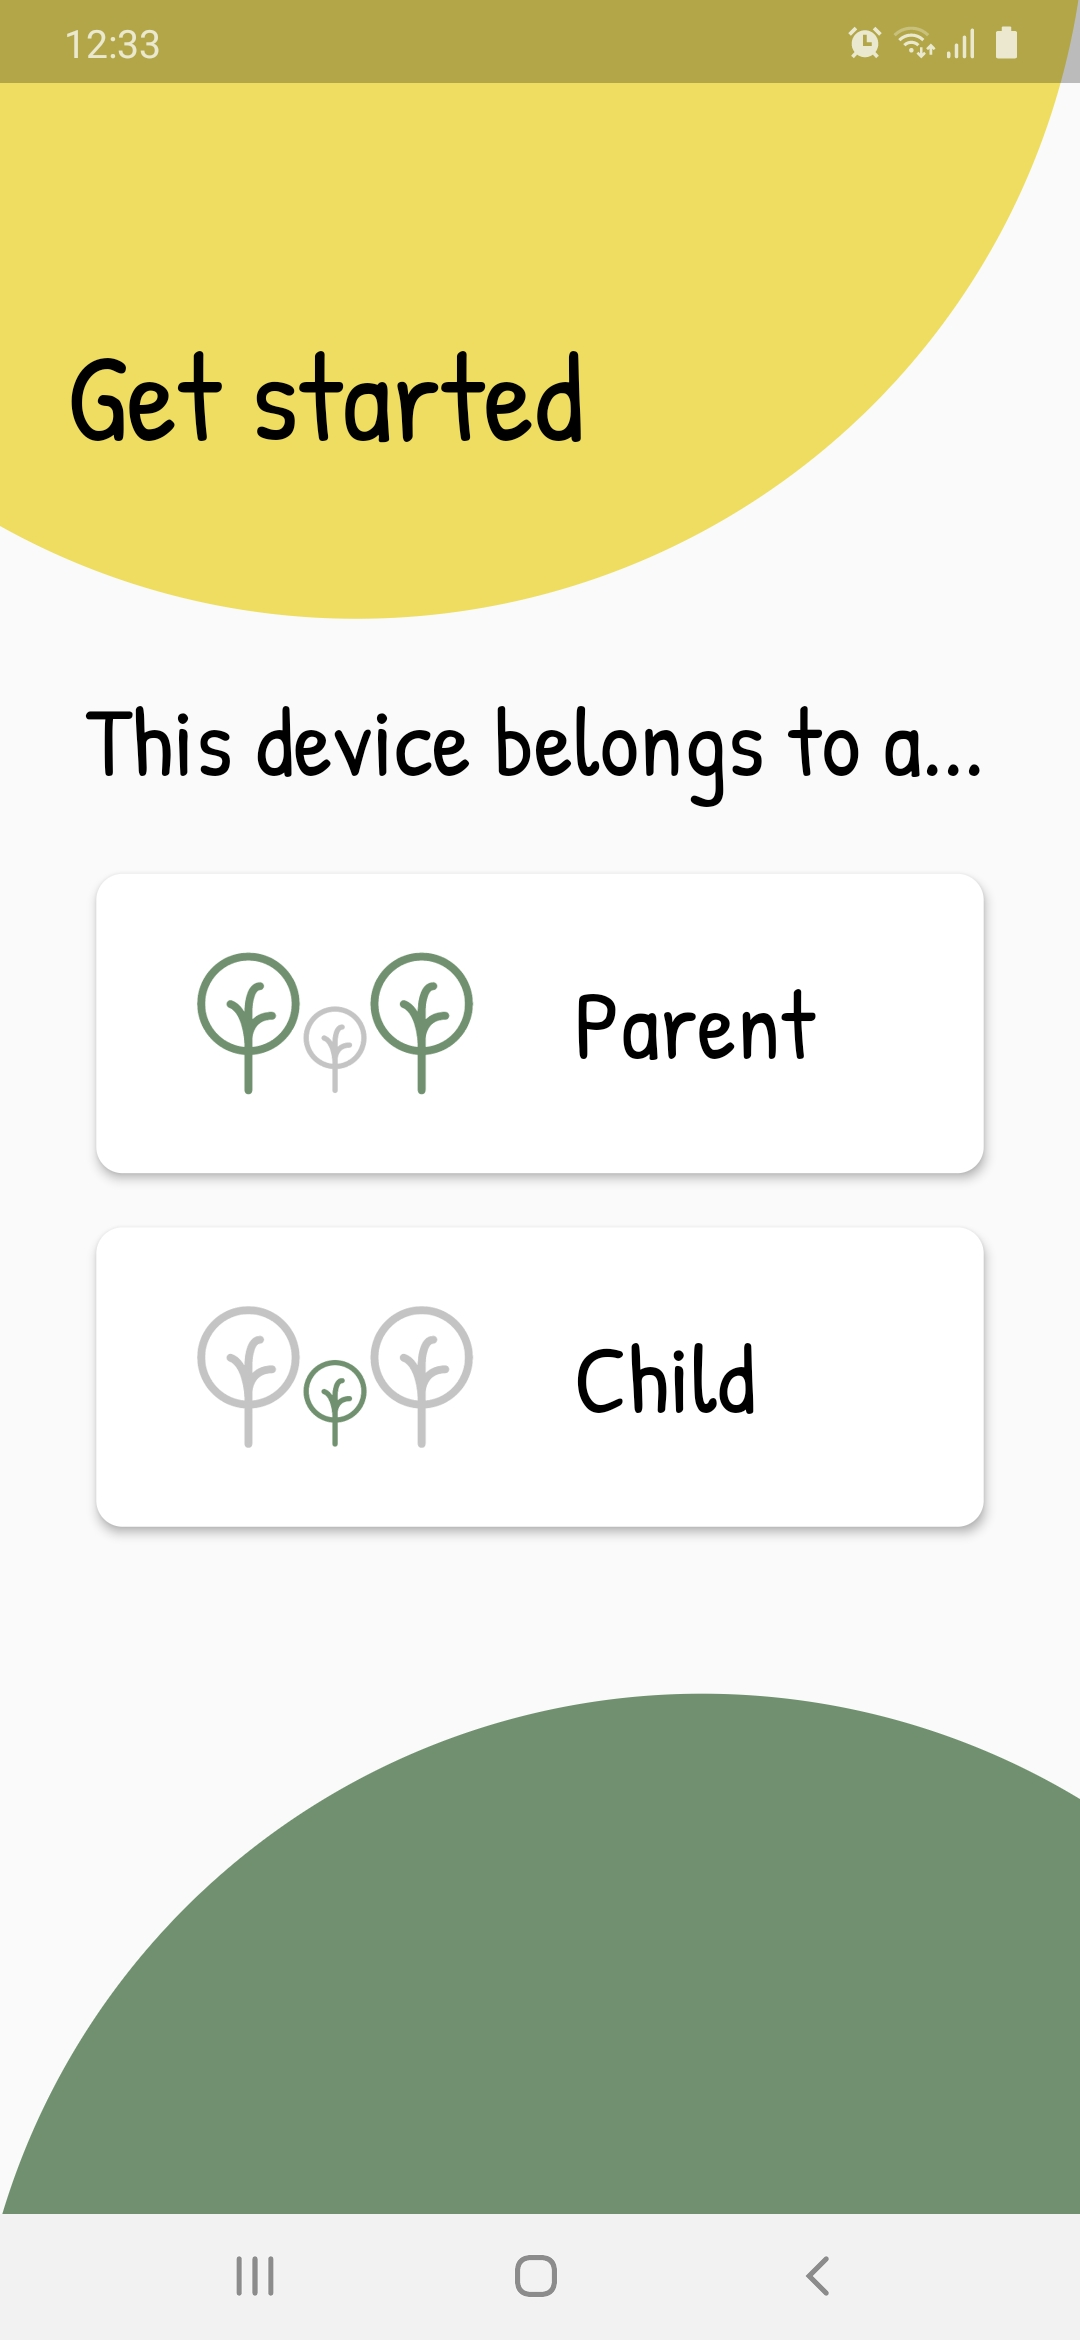
\includegraphics[width=.295\linewidth]{images/cross-device/SGA50/belonging.jpg}} 
&
\subcaptionbox{Login screen\label{fig:cross-device:sga50:login}}{ 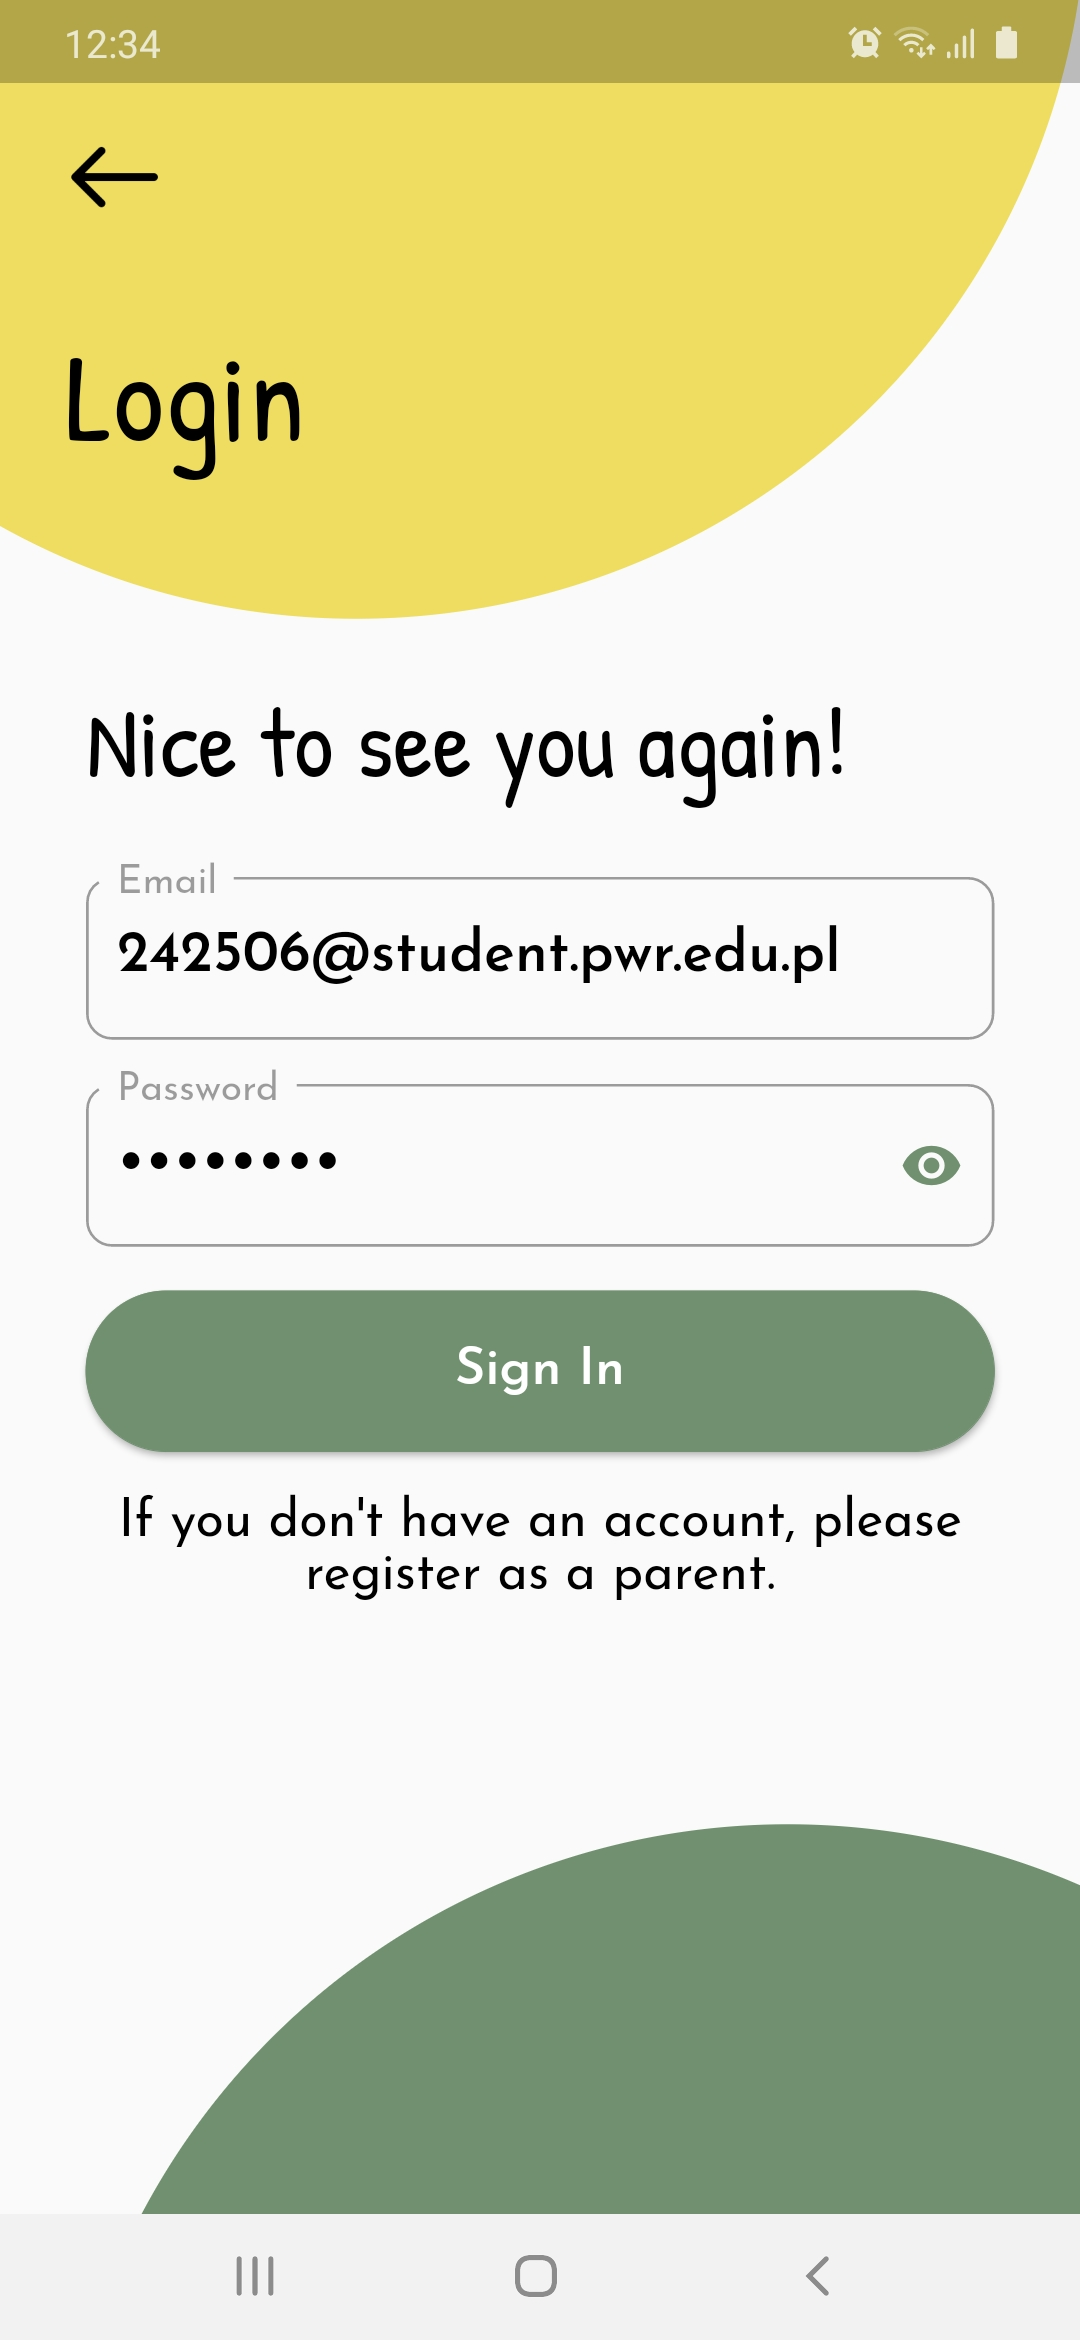
\includegraphics[width=.295\linewidth]{images/cross-device/SGA50/login.jpg}} 
&
\subcaptionbox{Children's profiles list screen\label{fig:cross-device:sga50:profiles}}{ 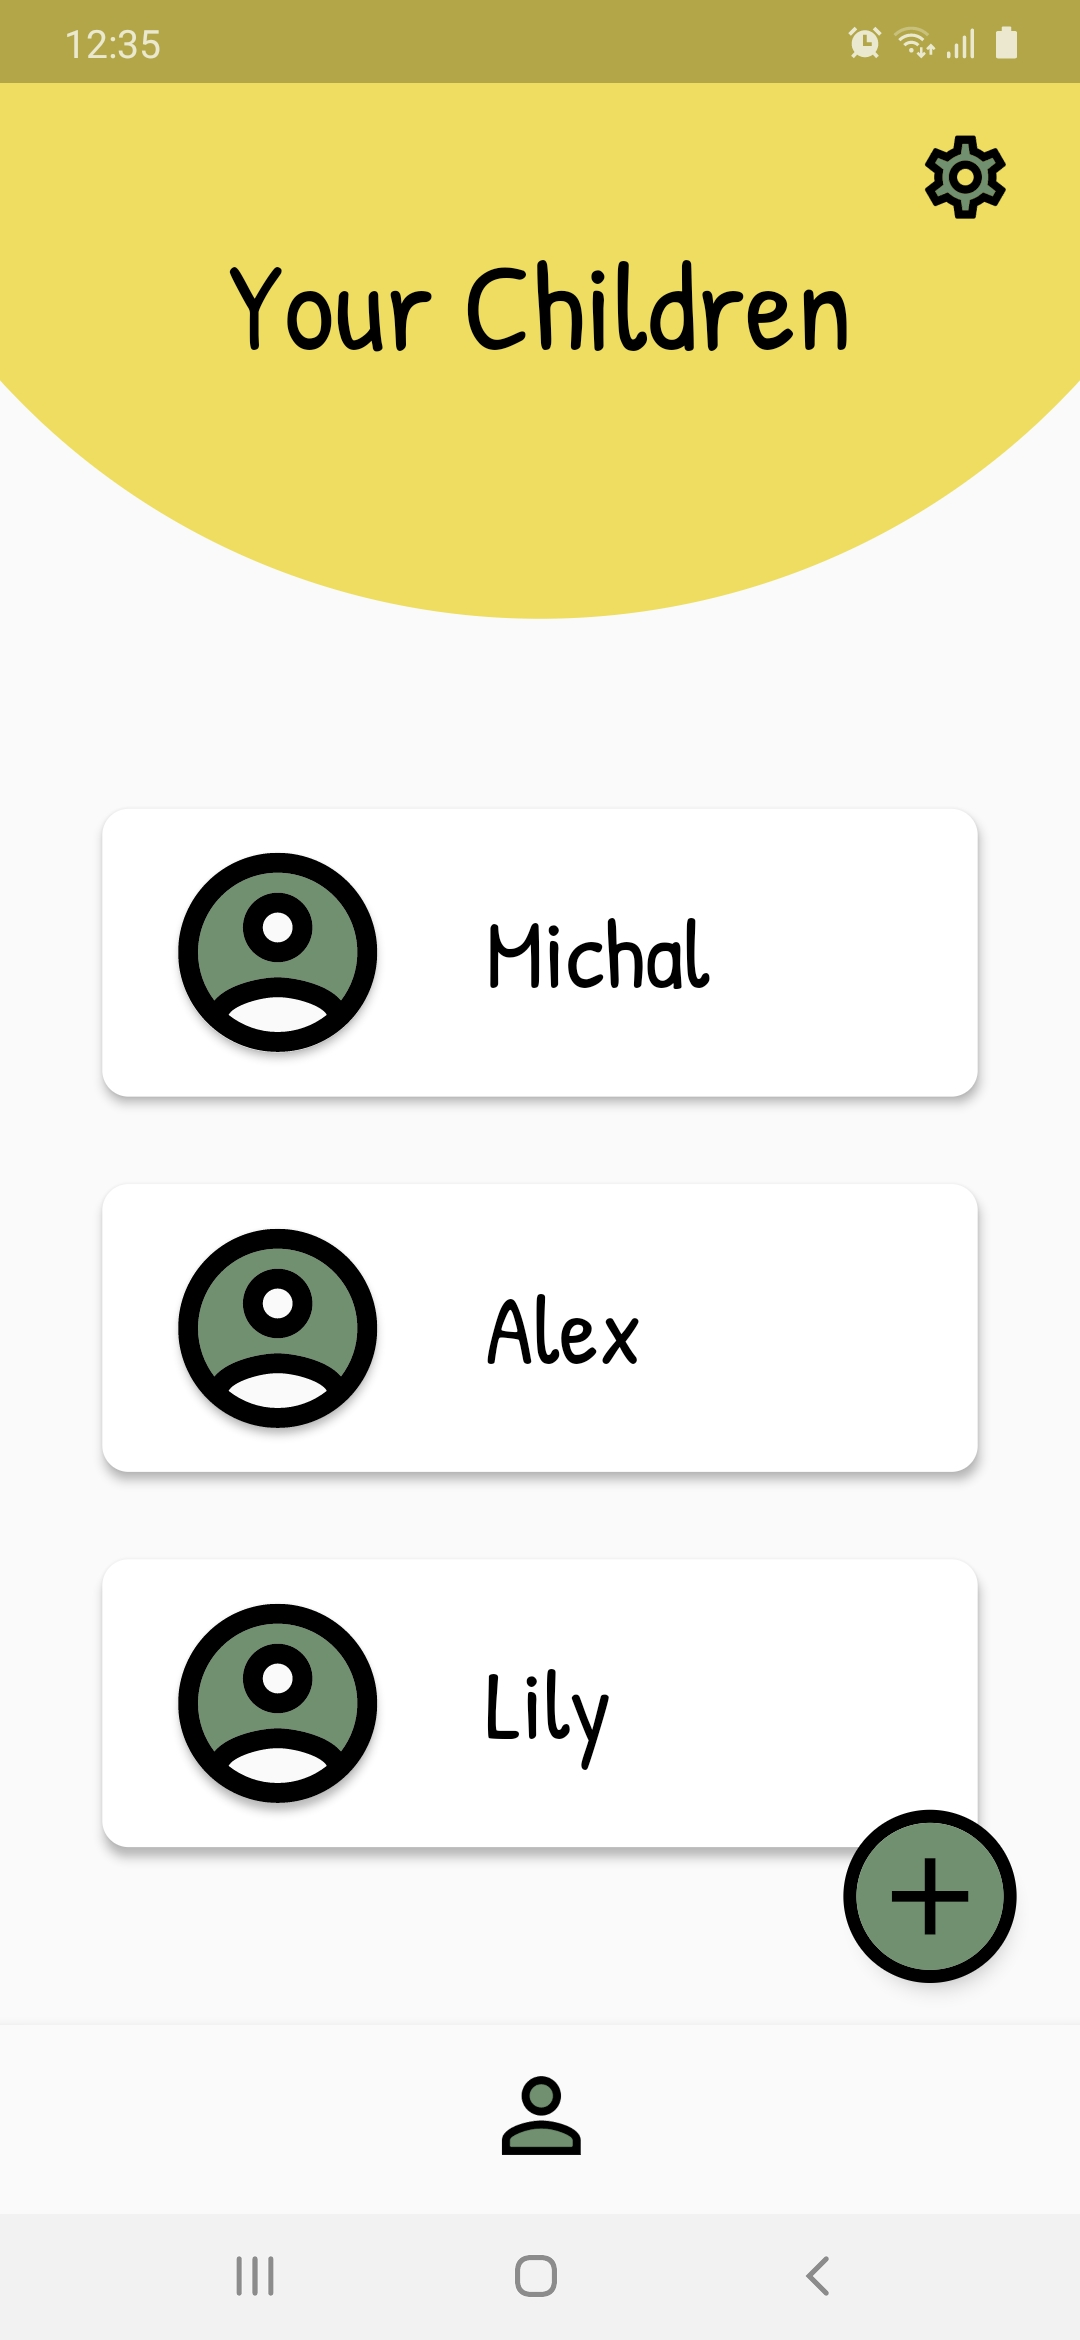
\includegraphics[width=.295\linewidth]{images/cross-device/SGA50/profiles.jpg}} 

\\\\\\\\
\subcaptionbox{Child's tasks screen\label{fig:cross-device:sga50:tasks}}{ 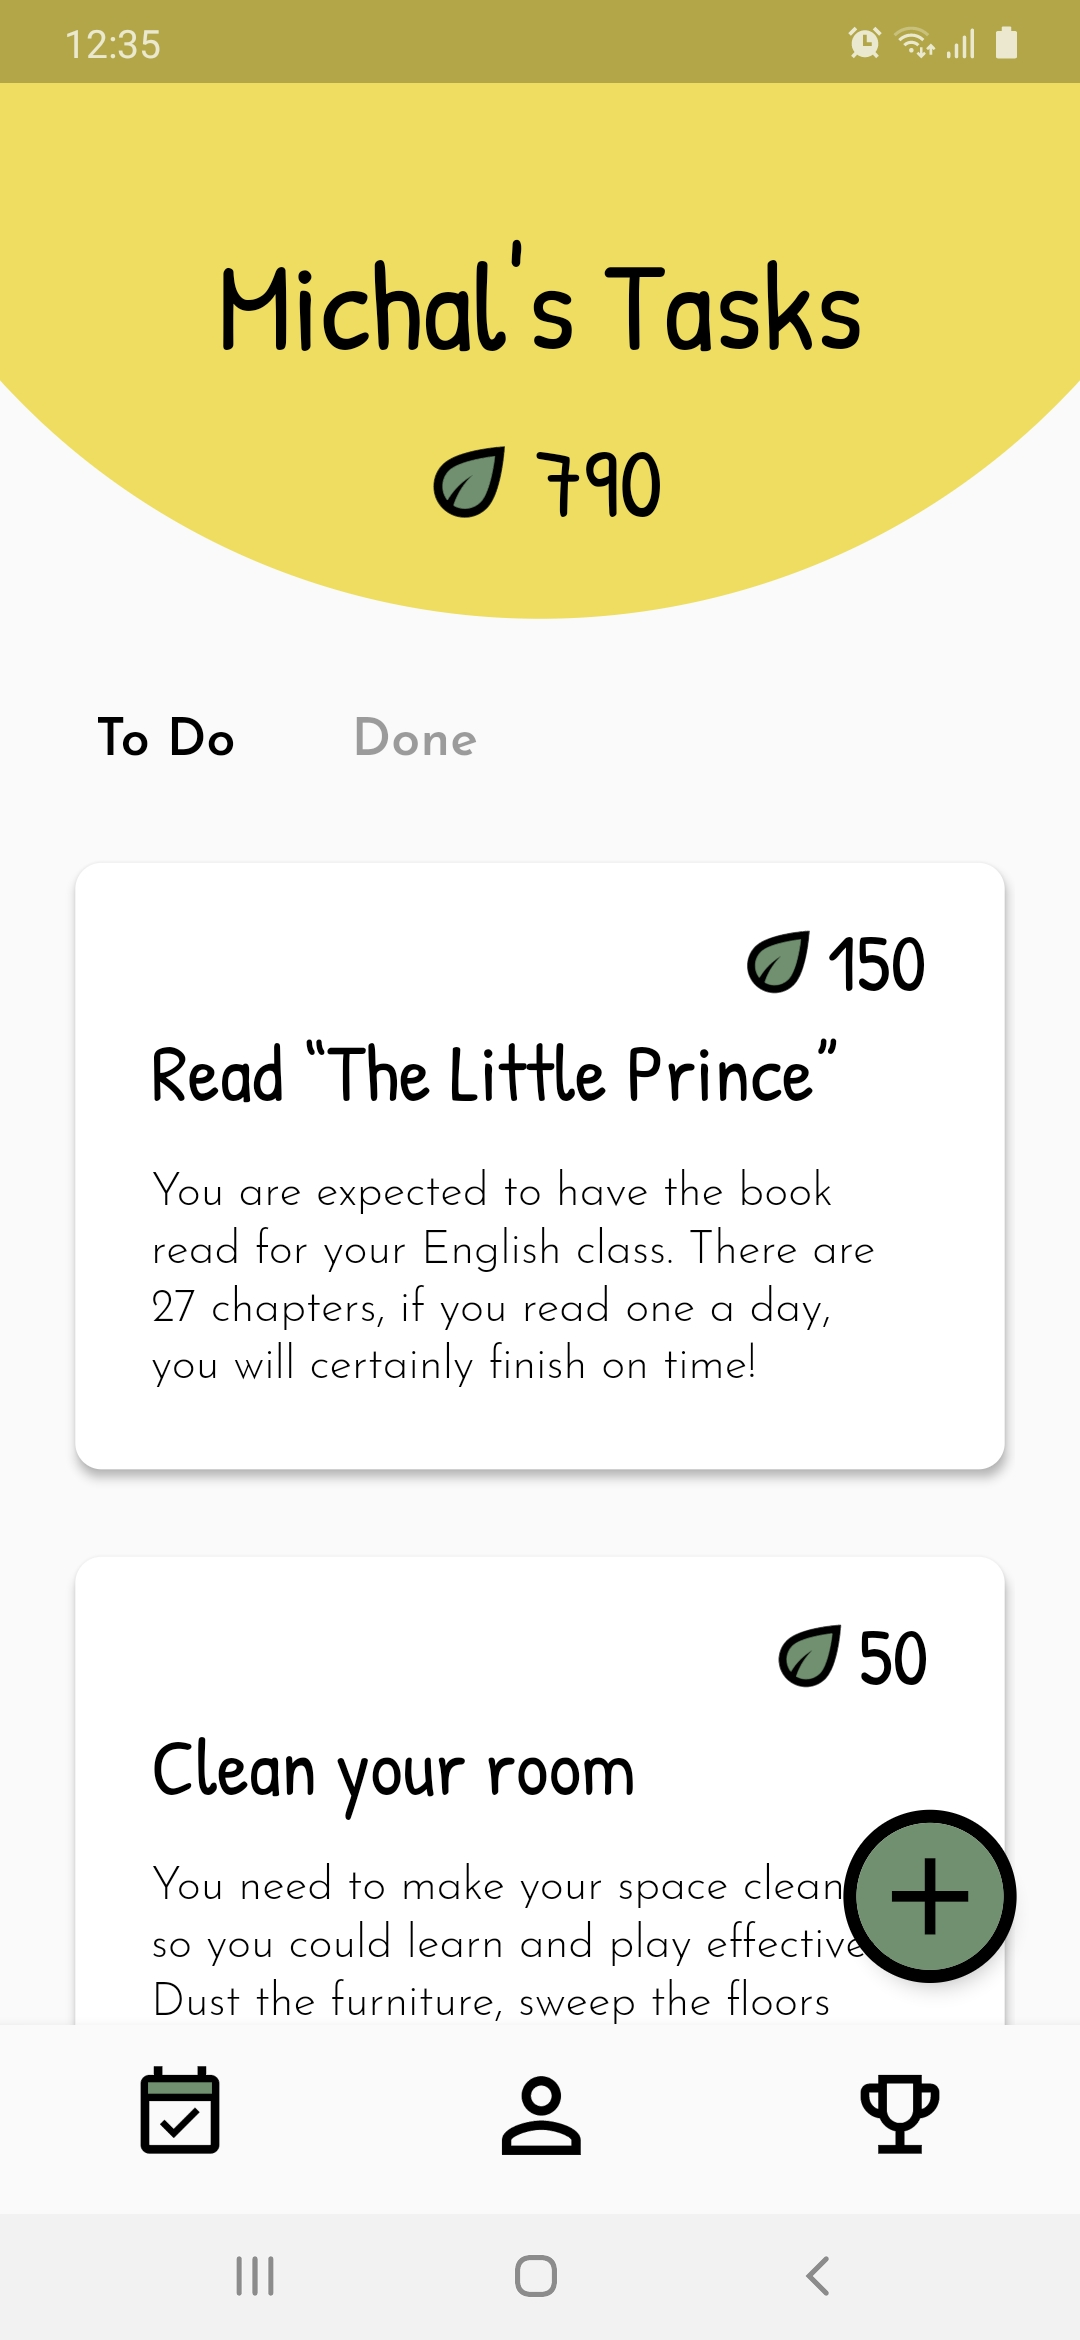
\includegraphics[width=.295\linewidth]{images/cross-device/SGA50/tasks.jpg}} 
&
\subcaptionbox{Task edit screen\label{fig:cross-device:sga50:edit-task}}{ 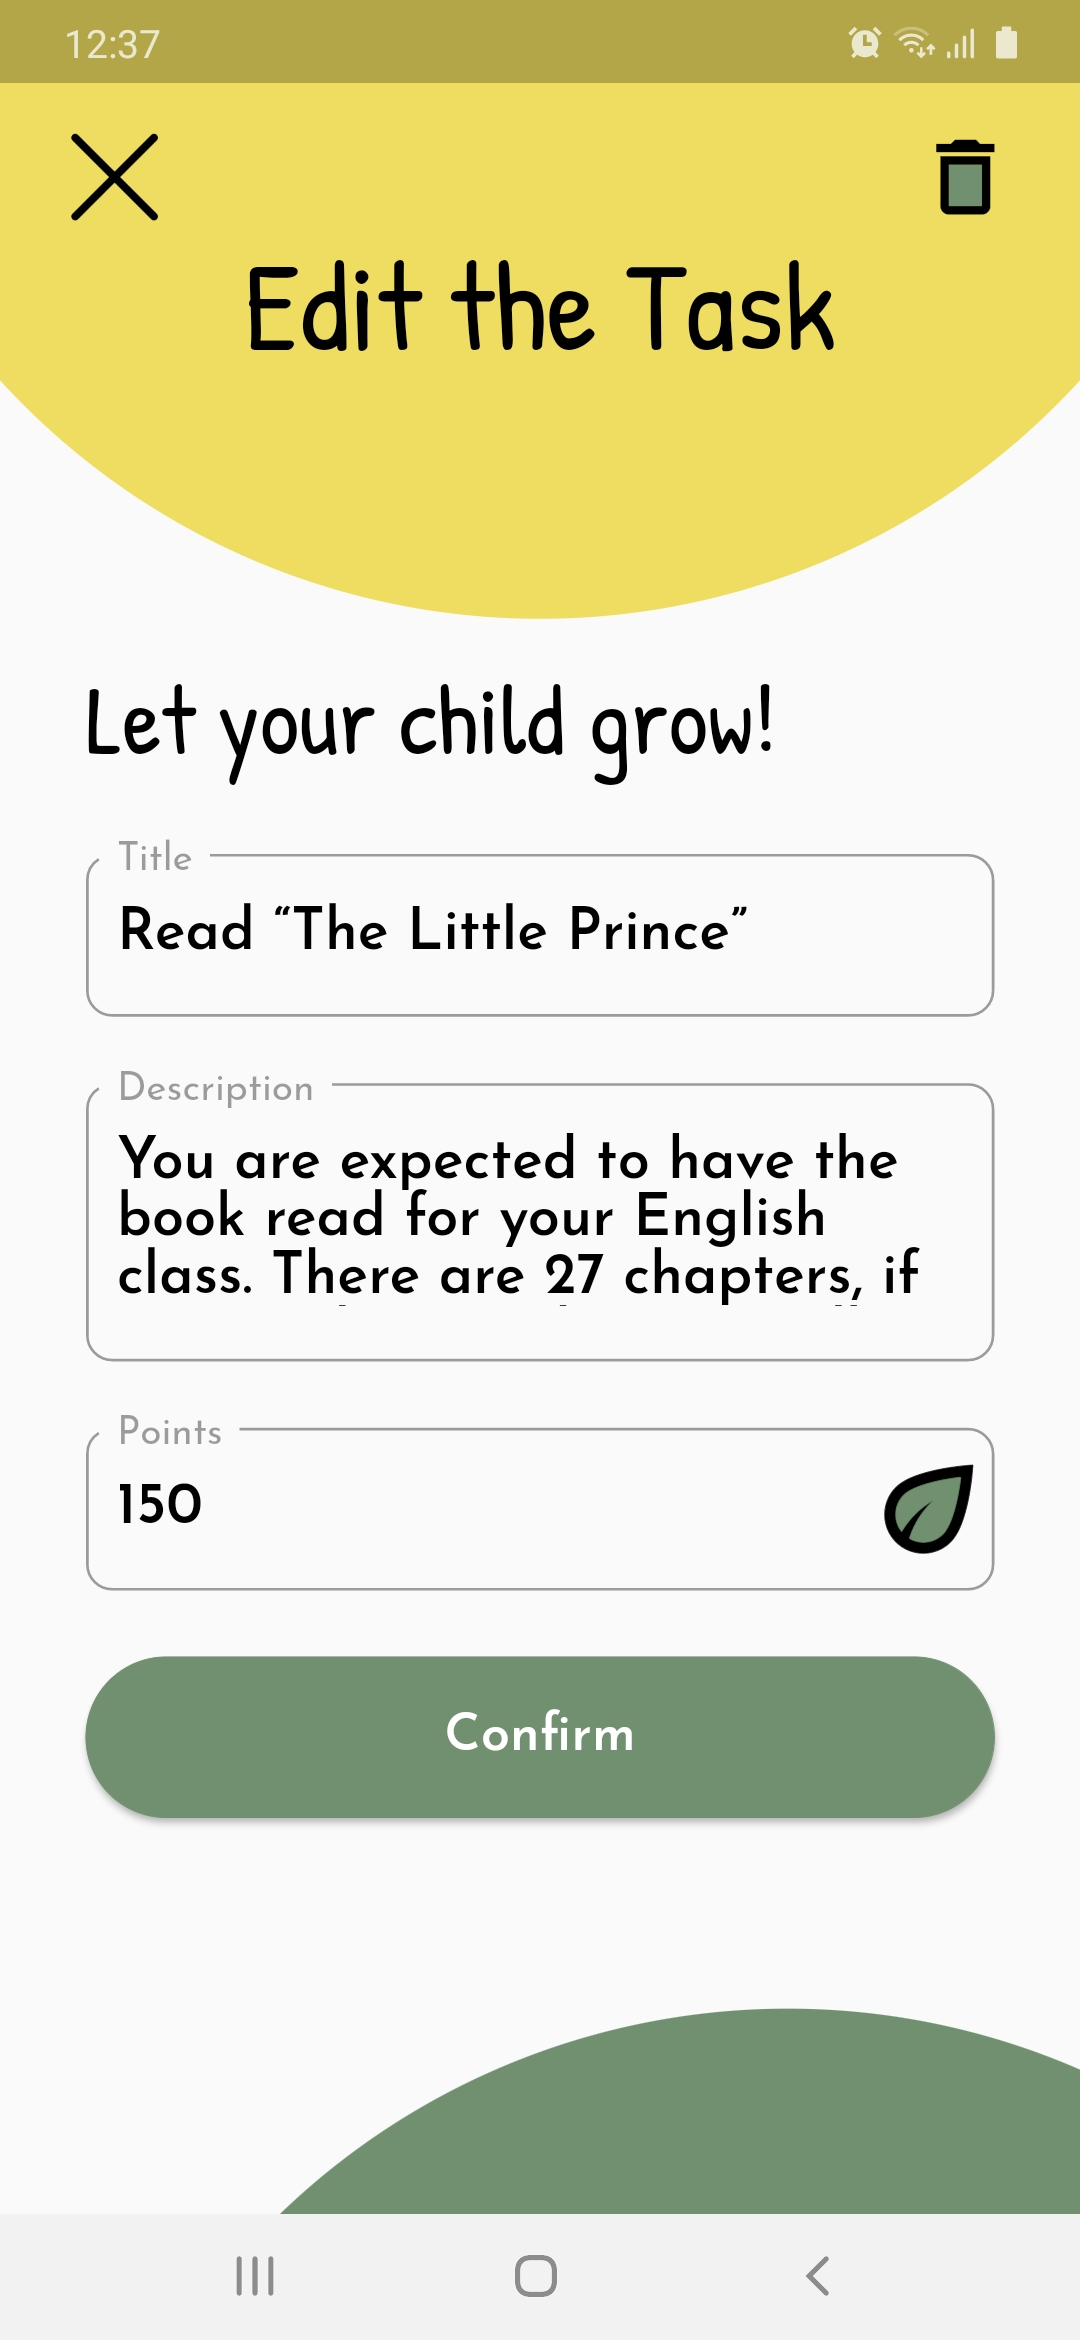
\includegraphics[width=.295\linewidth]{images/cross-device/SGA50/edit_task.jpg}} 
&
\subcaptionbox{Delete task confirmation\label{fig:cross-device:sga50:delete-task}}{ 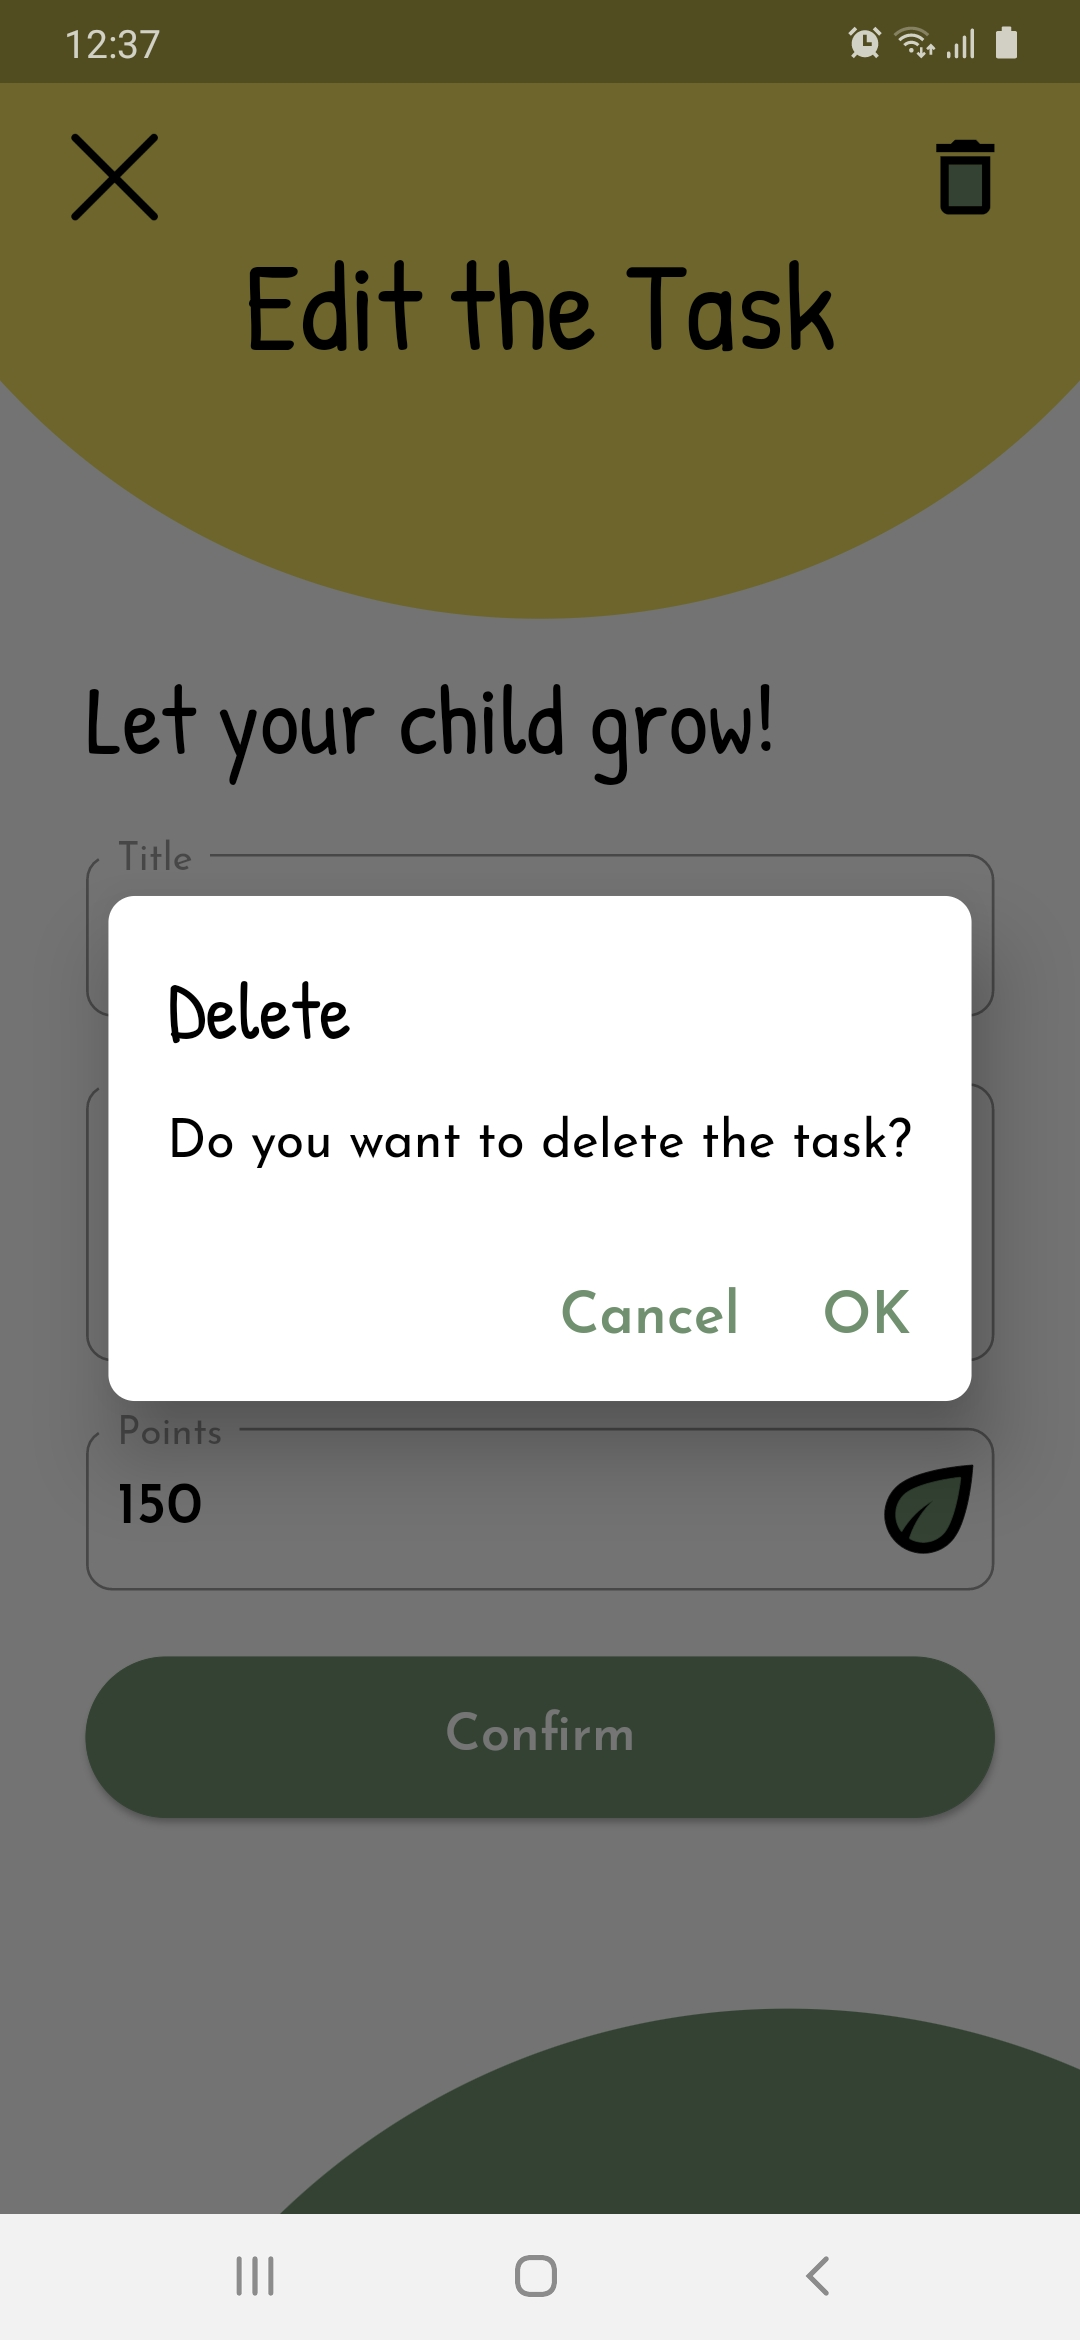
\includegraphics[width=.295\linewidth]{images/cross-device/SGA50/delete_task.jpg}} 
\end{tabular}
\caption{\textit{Raise App} selected screens displayed on Samsung Galaxy A50}
\label{fig:cross-device:sga50}
\end{figure}